\section{Modeling}
A model is a mathematical representation of a system that is determined by applying physical laws to a system and producing an equation.  The purpose of a model is to cut costs on the design because it is much less expensive to analyze an equation rather than a physical through trial and error.

An analytical model is created by determining the inputs and outputs of the system, which would include any type of signals going into the generator system and the effects the input has on the load.  Then, equations are developed based on known equations that represent the system.  Next, a transfer function is formed using the Laplace transform of the output of the system over the input.  This process is repeated for every input and output of the system.  From this model, critical system characteristics such as stability, accuracy, and speed can be optimized.  It is a good start seeing if a model will work in the real world with the transfer function \cite{analysis}.

An experimental model can be determined by collecting data output from a unit step input. This method produces more stable results because analytical models are based on ideal characteristics that are not entirely accurate for a real system. However, an experimental model has a higher cost due to expenses incurred for an accurate experiment. A typical design process would be to create an analytical model first, and then determine an experimental model in order to compare both models.

To obtain an accurate model for the generator system, a sequence of step response tests was performed, starting with an excitation voltage of 0.5 V and ending with a voltage of  5.0 V with increments of 0.5 V. It was observed that excitation voltages in the range from 1.5 V to 2.5 V produced terminal voltages in the desired range of 110 V. Figure \ref{fig:test_data} shows the results of the several step response tests.

\begin{figure}[h!]
\begin{center}
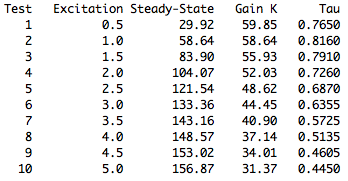
\includegraphics[scale=0.9]{./img/test_results.png}
\end{center}
\caption{Results of the step response tests}
\label{fig:test_data}
\end{figure}

One can obtain a first order transfer function model from the values of \begin{math}K\end{math} and \begin{math}\tau\end{math}. The equation for this model can be seen in eqn. \eqref{eq:tf_equation}:
\begin{equation}\label{eq:tf_equation}
G(s) = \frac{K}{1+\tau s}
\end{equation}

The modeled step responses were plotted and compared to the acquired data. Figure \ref{fig:model} shows an example plot of the recorded data and the calculated model for a excitation voltage of 2 V.
\begin{figure}[h!]
\begin{center}
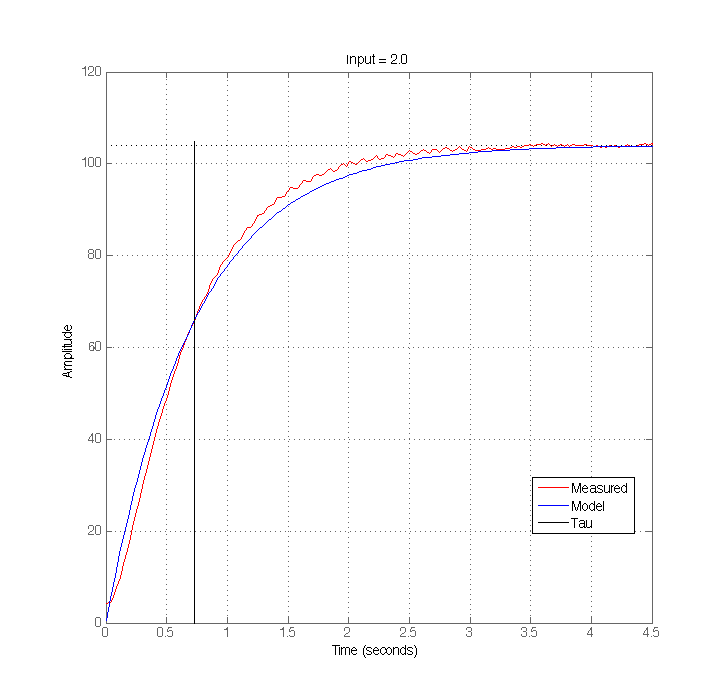
\includegraphics[scale=0.4]{./img/model.png}
\end{center}
\caption{Results of the step response tests}
\label{fig:model}
\end{figure}

We obtained our model by taking the arithmetic mean of the \begin{math}K\end{math} and \begin{math}\tau\end{math} values of the results of tests 3, 4, and 5. The resulting transfer function was:
\begin{equation}\label{eq:tf_model}
G(s) = \frac{52.19}{1+0.7347 s}
\end{equation}


